\chapter{Asking Holiday Shoppers How They Got RICH!}

This School of Hard Knocks interview, curated by LazyingArt LLC, proceeds less like a conventional lecture than like a sequence of field measurements. We begin with spectacle: cars, annual income figures, exits, ages. But the lecture does not stay there. It keeps asking what hidden structure produced those outcomes, and the answers return again and again to a small set of mechanisms: delayed gratification, recurring revenue, usable knowledge, capital access, sales, people, and execution. Since no validated board or slide images survived for this lecture, the equations below are cautious transcript-based reconstructions of the business arithmetic rather than transcriptions of visible mathematics.

\section{Hook, Montage, and the Houston Field Site}

The opening montage is a preview of variables before it is an argument. We hear large values --- \(\$194\) million, \(\$6\) million, \(\$8\) million, and an exit above \(\$740\) million --- but we are not yet told how these numbers fit together. The host then frames Houston, on his telling, as one of the world's richest cities and sets the method: we will move through the wealthiest shopping district, interview by interview, extracting mechanisms from visible outcomes.

To keep the lecture legible, we separate the main quantities from the start:
\begin{itemize}
\item \(Y_{\max}\): peak personal earnings in a single year;
\item \(C_{\text{rev}}\): company revenue;
\item \(E\): exit or sale value;
\item \(A\): current age;
\item \(A_{\$}\): age at first millionaire status;
\item \(T\): years spent in an industry or business.
\end{itemize}

This distinction is not bookkeeping for its own sake. It is the condition for reading the lecture properly. A company that did \(\$194\) million in revenue is not the same object as a founder who made \(\$6\) million in a year, and neither is the same as a company sold for more than \(\$740\) million.

\begin{table}[h]
\centering
\begin{tabular}{|l|l|l|l|}
\hline
Case & Quantity type & Reported value & Mechanism emphasized \\
\hline
Wealth management & \(Y_{\max}^{(\mathrm{wm})}\) & \(\$6\,\mathrm{M/yr}\) & Retainer, repeatability \\
Cybersecurity & \(M^{(\mathrm{cyber})}\) & \(\sim\) seven figures/month & Knowledge, protection \\
Energy & \(Y_{\max}^{(\mathrm{energy})},\,E^{(\mathrm{energy})}\) & \(\$8\,\mathrm{M/yr},\,>\$740\,\mathrm{M}\) & Capital, timing, risk \\
Lumber & \(C_{\text{rev}}^{(\mathrm{lumber},2022)}\) & \(\$194\,\mathrm{M}\) & People, delegation \\
\hline
\end{tabular}
\caption{Transcript-backed quantities that anchor the lecture's main case studies. The solar interview is used mainly for mechanism rather than for a clean numerical row, since its exact money figure is not reliably transcribed.}
\end{table}

The montage, then, is not the chapter itself. It is the index to the chapter. The first real development begins when the lecture chooses its most articulate case: a wealth manager whose answers are already organized around horizon, discipline, and revenue quality.

\section{Wealth Management and the Long Haul}

The first full interview begins by fixing a timescale. The speaker is in investment management and wealth management, has been in finance for \(40\) years, and corrects the host with quiet emphasis: he is not someone who \emph{was} in finance; he is still in it. Before we reach business structure, the lecture gives us a principle of temporal discipline. The best financial advice he received, he says, is that many people sacrifice what they want most for what they want now, and that ``now'' is an expensive word. The point is not asceticism. The point is that time horizon is already part of the mathematics.

He then supplies the first clean business profile. Yes, he owns a business. He started his own wealth-management firm \(13\) years ago, and it has grown to about seven times the size of the brokerage practice he left. His best single year was
\[
Y_{\max}^{(\mathrm{wm})}=\$6\,\mathrm{M/yr}.
\]
So before the lecture has yet given us its explicit blueprint, it has already given us three things: a long horizon, a business he owns, and a revenue stream capable of compounding beyond salaried or deal-by-deal labor.

The speaker's advice about hanging in for the long haul is therefore not detachable from the later discussion of recurring revenue. The lecture is moving toward a structural claim, but it first wants us to feel the duration required to make that claim meaningful.

\section{From Rock Bottom to the Blueprint}

The lecture now performs one of its most important turns. It does not move immediately from \(\$6\) million to a formula. It moves back into biography. The speaker says that he spent the first half of his life broke, came from a divorced household, came from nothing, and saw his mother's car repossessed. In the spoken rhythm of the interview, this is not decorative sentiment. It is the ground from which the later blueprint becomes credible.

\subsection{Question \& Answer}

What can someone at rock bottom do right now?

The host asks this directly, and the answer is not a trick, not leverage masquerading as spirituality, and not a secret industry tip. The answer is a sequence of disciplines: go to church, pray, learn, be curious, figure out how things work, and learn how to articulate that understanding to other people. The last step matters. Knowledge that cannot be made socially intelligible does not yet create trust.

This is where the lecture's moral vocabulary and its business vocabulary meet. People seek out those who are both knowledgeable and trustworthy. In the logic of the chapter, trust is not an ornament added after scale; it is one of the preconditions for scale.

Only after this does the lecture return to chronology. The speaker is now \(64\) years old, and he became a millionaire at
\[
A_{\$}^{(\mathrm{wm})}=36.
\]
So the lecture has now established a whole trajectory: long financial apprenticeship, hard personal origins, a late-enough but still very significant wealth threshold, and a business architecture that can repeat.

\subsection{Question \& Answer}

Why does recurring, non-transactional revenue scale better than one-off deal flow?

Now we reach the cleanest analytical moment in the lecture. Asked for a blueprint for a young viewer who wants to become a millionaire, the speaker says we should think about businesses that generate recurring revenue and do so in a non-transactional way. He contrasts this with commercial real estate: one can make a great deal of money there, but one must repeatedly go out and find the next deal.

We can formalize that contrast in deliberately simple notation:
\begin{align}
R_{\text{trans}} &\approx N_d f_d, \\
R_{\text{rec}} &\approx N_c\,p\,H\,\rho.
\end{align}
Here \(N_d\) is the number of deals and \(f_d\) the average value per deal, while \(N_c\) is the number of recurring clients, \(p\) the payment per period, \(H\) the horizon, and \(\rho\) a persistence factor capturing retention.

\begin{definition}
A transactional revenue stream is one in which each increment of income requires a fresh deal, a fresh search, or a fresh closing event.
\end{definition}

\begin{definition}
A recurring revenue stream is one in which the client relationship persists across billing periods, so that acquisition effort is not fully restarted each time income arrives.
\end{definition}

The interview then gives us a concrete example. The speaker says that one set of transactions can be delivered and applied to \(100\) different people, and those \(100\) people all pay for it. This is the lecture's clearest statement of scalable replication.

\begin{figure}[h]
\centering
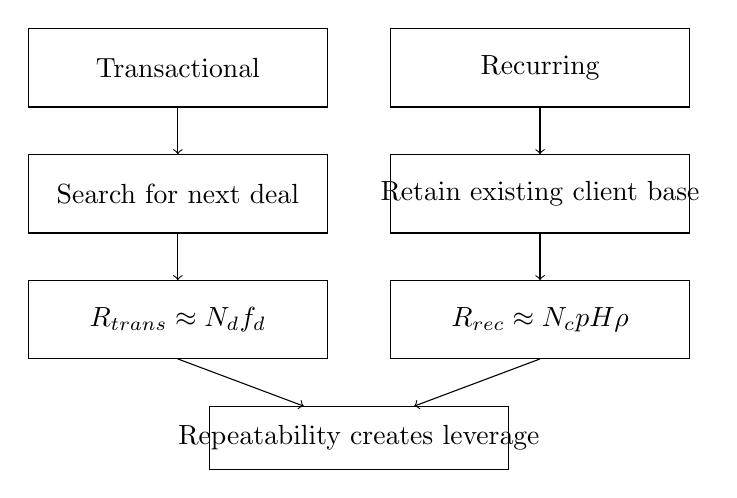
\begin{tikzpicture}[x=1cm,y=1cm]
\draw (0,0) rectangle (3.8,1) node[pos=.5] {Transactional};
\draw (4.6,0) rectangle (8.4,1) node[pos=.5] {Recurring};

\draw (0,-1.6) rectangle (3.8,-0.6) node[pos=.5] {Search for next deal};
\draw (4.6,-1.6) rectangle (8.4,-0.6) node[pos=.5] {Retain existing client base};

\draw (0,-3.2) rectangle (3.8,-2.2) node[pos=.5] {\(R_{\text{trans}}\approx N_d f_d\)};
\draw (4.6,-3.2) rectangle (8.4,-2.2) node[pos=.5] {\(R_{\text{rec}}\approx N_c p H \rho\)};

\draw[->] (1.9,0) -- (1.9,-0.6);
\draw[->] (1.9,-1.6) -- (1.9,-2.2);
\draw[->] (6.5,0) -- (6.5,-0.6);
\draw[->] (6.5,-1.6) -- (6.5,-2.2);

\draw (2.3,-4.6) rectangle (6.1,-3.8) node[pos=.5] {Repeatability creates leverage};
\draw[->] (1.9,-3.2) -- (3.5,-3.8);
\draw[->] (6.5,-3.2) -- (4.9,-3.8);
\end{tikzpicture}
\caption{Editorial schematic of the lecture's central comparison. No visual board evidence survives for this lecture; the figure is a transcript-based reconstruction of the contrast the speaker draws.}
\end{figure}

\begin{proposition}
Under the lecture's own assumptions, a repeatable retained service can outgrow a purely transactional model because client count and retention multiply the same underlying process across time.
\end{proposition}

\begin{proof}
The derivation is short.
\begin{enumerate}
\item In a purely transactional model, each unit of income is tethered to a fresh deal, so revenue is approximately \(R_{\text{trans}} \approx N_d f_d\).
\item In the retained model described in the lecture, we build one common service bundle and deploy it across many clients.
\item The transcript gives \(N_c \approx 100\) as a concrete scale example.
\item If each of those clients pays \(p\) per period across horizon \(H\) with persistence \(\rho\), then
\[
R_{\text{rec}}^{(100)} \approx 100\,p\,H\,\rho.
\]
\item The decisive feature is not merely that \(100\) is a large number. It is that the service architecture is reused rather than rebuilt from zero.
\end{enumerate}
Hence, once marginal delivery cost is sufficiently low and retention sufficiently strong, the lecture's intuitive conclusion follows:
\begin{equation}
R_{\text{rec}}(H) > R_{\text{trans}}(H)
\end{equation}
for a sufficiently long horizon \(H\).
\end{proof}

The host immediately pauses to extract the theorem-like moral: recurring revenue is the way to go, and it is striking precisely because, in his telling, this is not what school usually teaches. The interview then closes this arc with a character question --- what trait do highly successful people share? --- and the answer returns to fidelity, focus, and doing the right thing. So the blueprint is not merely structural. It is structural plus durable character. That is how the lecture wants us to connect trust and revenue.

\section{Cybersecurity, Ignorance, and Time Compression}

The host now changes tempo. He recaps the finance lesson in slogan form and then resets the scene with a G-Wagon and a younger founder. The new speaker started a cybersecurity company, says the business is doing roughly seven figures a month, is \(27\) years old, and became a millionaire this year. The lecture is deliberately placing a fast-growth case after a long-horizon case. It wants to know what can be sped up and what cannot.

The first answer is blunt: what keeps people broke is ignorance. But the speaker immediately clarifies that ignorance is not some metaphysical curse. It is simply lack of the knowledge relevant to the result one wants. He then says that one can collapse time through knowledge.

We should state that carefully. The lecture is not claiming that time literally disappears. It is claiming that failed search can be shortened. A clean reconstruction is
\begin{align}
t_{\text{reach}} &= t_{\text{search}} + t_{\text{execution}}, \\
\frac{\partial t_{\text{search}}}{\partial K} &< 0,
\end{align}
where \(K\) is usable knowledge imported from mentors, models, or operators who have already achieved the target state.

\subsection{Question \& Answer}

How does knowledge collapse time?

The answer is that the route becomes less expensive to discover. In the lecture's own sequence, the derivation is almost procedural:
\begin{enumerate}
\item Decide where we want to go.
\item Assume that someone else has already gotten there.
\item Learn what that person did.
\item Stop reinventing steps whose cost has already been paid by others.
\end{enumerate}
So the phrase ``collapse time'' should be read as a business-timescale heuristic: imported knowledge lowers search cost and eliminates avoidable dead ends.

The founder then gives the lecture a second layer. Asked what industry people should be looking at going into \(2024\), he answers, unsurprisingly, cybersecurity. His reason is not fashion. It is that protecting organizations is economically valuable, and protection is a capability companies will pay for. This keeps the lecture honest. We are not being told to admire entrepreneurship in the abstract; we are being told to look for costly problems and scarce skills.

The interview then loops back to hardship. He says he was broke only a few years before, and when asked about the turning point, he answers that he stopped making decisions alone. Everywhere he wanted to go, someone had already gone, so the sensible move was to find those people and follow the path they had already tested. The host's recap after this segment is again pedagogically important: the money lesson becomes a knowledge lesson. Resourcefulness matters more than the mere presence of resources.

\section{Energy, Capital Access, and Timing}

The next interview widens the frame from knowledge and sales to finance, ownership, and risk. The speaker chose energy, oil, and gas, has been in the business for \(35\) years, reports a best single year of
\[
Y_{\max}^{(\mathrm{energy})}=\$8\,\mathrm{M/yr},
\]
and says the company sale was
\[
E^{(\mathrm{energy})}>\$740\,\mathrm{M},
\]
with the transcript preserving some contingent language around a possible higher endpoint. He is now \(65\), and he says he only became a millionaire about five years ago. The lecture is again forcing a distinction between current visible wealth and the timing by which that wealth was actually realized.

The most conceptually important answer in this section comes when the host asks what he would do differently if he could start over. He says he would start in banking.

\subsection{Question \& Answer}

Why can capital literacy matter more than pure technical specialization?

The energy founder's answer is subtle. Technical geophysics and geology are good, but they often leave one working for someone else. Banking, by contrast, teaches where money comes from, who controls it, and how the relevant structures fit together. In the language of these notes, finance enlarges the feasible set:
\begin{equation}
\mathcal{F}_{\text{technical}} \subset \mathcal{F}_{\text{capital}}.
\end{equation}
Here \(\mathcal{F}_{\text{technical}}\) is the set of moves available to a purely technical operator, while \(\mathcal{F}_{\text{capital}}\) is the larger set available once one understands funding, ownership, and deal structure.

The lecture's next move is from capital literacy to timing. Asked what took the business from eight figures to nine, the answer is not ``genius'' but progressive risk, very hard work, and getting in at the right time, specifically when Mexico opened up and the team drilled an early well that came in large. We should resist flattening this into generic risk-taking. The lecture's logic is that timing matters because opportunity is not evenly available across all moments; some market openings produce a discontinuous expansion of payoff.

The final advice in this section turns from money back to people: study, talk to people, work with good people, trust those with whom we build. The speaker even frames action in ripple terms: one good act, one good decision, or one correctly executed effort can have effects beyond its immediate local setting. The host's recap then distills the case into a stark summary: long play inside the same game, expertise accumulated over decades, and a nine-figure exit.

\section{Solar Sales, Team Structure, and the Mentor Principle}

The lecture now pivots from oil and gas to solar, and the mood changes again. The speaker owns a solar company, and when asked how he scaled from six to seven figures, he does not answer first with product or market. He answers with people. If we want to go farther, he says, we go with people together. He then describes an internal structure with leadership, sales, marketing, and channels of mutual accountability.

This is also the moment when the lecture gives its strongest defense of commission sales. The speaker says plainly that if one wants to make money in the United States, one need not romanticize entrepreneurship; one can go into commission sales. In minimal form we may write
\begin{equation}
Y_{\text{sales}} \approx N_s c,
\end{equation}
where \(N_s\) is the number of successful closes and \(c\) is the average commission per close. This is, again, an editorial reconstruction rather than transcript notation, but it captures the argument. Sales skill is itself a revenue engine.

The interview's personal material matters here as well. The speaker describes coming from Honduras, arriving in the United States young without speaking the language, struggling, entering sales, and eventually doing well financially. Some of the transcript is garbled, but the mechanism is clear: sales widened access to people, people widened access to opportunity, and disciplined work converted that access into income.

The lecture then returns to people in a second sense. If we take care of our people, they take care of the business. This brings us close to the final lumber lesson, but not yet all the way there. Here the emphasis is still on team formation and the commercial power of being good with people.

A final warning closes the section. The speaker says he is not interested in becoming a social-media personality; he wants to make money in a way that allows him to disappear. Hence the distinction between mentor and guru. Information is abundant --- one can search, learn, and cross-check cheaply --- but a mentor is different from a performer. The lecture's deeper claim is that public visibility and economic substance are not the same variable.

The host's recap makes the point sharply: the man in the Lamborghini did not begin there. He began broke, learned how to sell, invested in himself, and built from there.

\section{Lumber, Delegation, and Execution}

The final major case turns the lecture from skill acquisition to operating scale. The speaker is in the lumber industry, says that in \(2022\) his company did
\[
C_{\text{rev}}^{(\mathrm{lumber},2022)}=\$194\,\mathrm{M},
\]
and reports that he became a millionaire at \(35\). When the host asks what took the company from eight figures to nine, the answer comes at once: identifying people.

That answer is then sharpened. The speaker says he is not really in the lumber business; he is in the people business. He does not believe in hiring someone to do the owner's job, but he does insist that at scale one must let go of certain things. The business owner cannot be worrying about the price of toilet paper.

\subsection{Question \& Answer}

What takes a company from eight figures to nine?

The lecture's answer is people, delegation, and execution. A useful editorial compression is
\begin{equation}
S \approx P\,\Gamma\,X,
\end{equation}
where \(S\) is scale, \(P\) is people quality, \(\Gamma\) is coordination and delegation capacity, and \(X\) is execution quality. This is not the lecture's notation; it is our way of keeping its logic in one line.

The derivation is operational rather than abstract:
\begin{enumerate}
\item At small size, the founder can perform many functions directly.
\item As the firm grows, owner attention becomes scarce.
\item If the owner refuses to release local tasks, owner attention becomes the bottleneck.
\item Hiring strong people raises \(P\).
\item Giving those people real operating room raises \(\Gamma\).
\item Follow-through, precision, and focus raise \(X\).
\item Therefore the system, not merely the founder's willpower, determines the next scale threshold.
\end{enumerate}

The speaker then gives the lecture its final sentence of business ethics: ideas are cheap; execution is everything. When the host presses him to explain, he expands execution into follow-through, precision, and focus. Originality is not the scarce resource. Competent realization is.

This ending is strong precisely because it strips away the glamour that opened the video. We began with cars. We end with toilet paper, delegation, and the disciplined narrowing of a founder's attention.

\section{Summary}

The lecture unfolds as a controlled sequence of recalibrations. First it lures us with visible wealth. Then it shows us that the meaningful variables are different: horizon, trust, recurring revenue, imported knowledge, capital access, sales skill, team quality, and execution. The first finance interview gives the chapter its clearest business arithmetic; the cybersecurity interview shows how borrowed knowledge shortens the path; the energy interview shows why finance widens the set of possible moves; the solar interview insists on commission sales and mentorship; and the lumber interview closes with delegation and operational discipline.

If we compress the chapter to a single progression, it is this. We first learn not to confuse numbers with mechanisms. We then learn that trust and delayed gratification make recurring revenue possible. We next learn that knowledge lowers search cost and that capital literacy widens the feasible set. Finally, once the business grows, we learn that people and execution govern scale more than ideas alone. That is the mathematical payload of the lecture: not formal theory for its own sake, but a serious arithmetic of leverage, persistence, and organized action.